\documentclass{beamer}

\usepackage[T1]{fontenc}
\usepackage[english]{babel}
\usepackage[utf8]{inputenc}
\usepackage{graphicx}
\usepackage{textcomp}

% Add the citation package
\usepackage[alf,abnt-emphasize=bf]{abntex2cite}

% Choose the Inf theme
\usetheme{Inf}

% --- Title Information ---
\title[HIoT Data Security with MA-ABE]{A Hybrid Multi-Authority Attribute-Based Encryption Scheme For Securing HIoT Data}
\author{Felipe de Almeida Graeff}
\institute{Instituto de Informática --- UFRGS \\ \vspace{0.5cm} Advisor: Prof. Dr. Jéferson Campos Nobre \\ Co-advisor: M.Sc Laura Rodrigues Soares}
\date{8 de julho de 2025}

\begin{document}

% --- Title Page ---
\begin{frame}[plain]
\titlepage
\end{frame}

% --- Agenda ---
\begin{frame}
\frametitle{Agenda}
\tableofcontents
\end{frame}

% --- Introduction ---
\section{Introduction}

\begin{frame}
\frametitle{Background}
\begin{figure}
    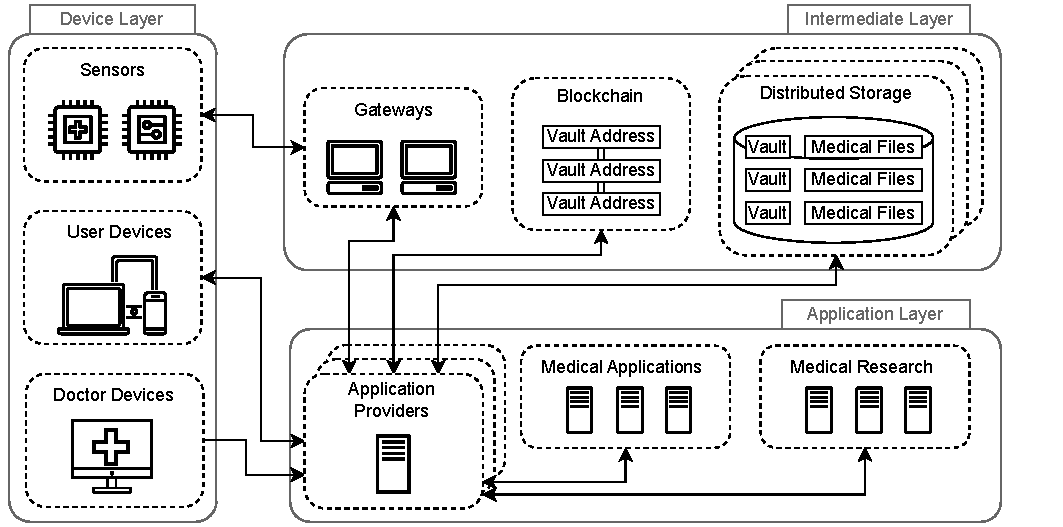
\includegraphics[width=\textwidth,height=0.7\textheight,keepaspectratio]{images/diagrams/fig2-grefo.drawio.pdf}
    Framework proposed by \citeonline{laura2023} for decentralized HIoT data storage.
\end{figure}
\end{frame}

\begin{frame}
\frametitle{Context: The Explosion of Data in HIoT}
\begin{itemize}
    \item Massive adoption of devices performing continuous, real-time monitoring of vital signs.
    \item Generation of an unprecedented volume of Electronic Health Records (EHRs).
    \item Inclusion of highly complex and sensitive data, such as genomic information and medical imaging.
    \item This scenario results in a data ecosystem with unprecedented volume, variety, and sensitivity.
\end{itemize}
\end{frame}

\begin{frame}
\frametitle{Context: Vulnerabilities of the Centralized Model}
\begin{itemize}
    \item Consolidated health data represents an extremely valuable target for cyberattacks.
    \item Traditional architectures based on centralized servers create a single point of failure.
    \item A single security breach can lead to the mass exposure of confidential data from millions of patients.
    \item The centralized model is therefore inherently inadequate to provide the security required by HIoT systems.
\end{itemize}
\end{frame}

\begin{frame}
\frametitle{Context: The Need for a New Security Paradigm}
\begin{itemize}
    \item \textbf{Confidentiality:} Ensuring that only authorized entities can view the data.
    \item \textbf{Integrity:} Ensuring that data has not been improperly altered or corrupted.
    \item \textbf{Fine-Grained Access Control:} Implementing granular and dynamic access policies based on user attributes (e.g., 'doctor,' 'researcher,' 'hospital').
    \item The demand is for a security framework that is simultaneously robust, flexible, and efficient for the healthcare ecosystem.
\end{itemize}
\end{frame}

\begin{frame}
\frametitle{Problem Statement}
\begin{itemize}
    \item Existing decentralized HIoT architectures, often lack a concrete cryptographic layer for end-to-end data confidentiality and fine-grained access control.
    \item Traditional encryption methods offer binary ("all-or-nothing") access, which is insufficient for the complex, multi-stakeholder healthcare environment requiring dynamic, attribute-based permissions.
    \item Advanced cryptographic schemes like Attribute-Based Encryption (ABE) can introduce significant computational overhead, posing performance and scalability challenges for real-world HIoT systems.
    \item The complexity of many ABE schemes makes rigorous security verification difficult, creating a need for a carefully selected and robustly implemented solution to ensure trustworthiness.
\end{itemize}
\end{frame}

% --- Proposed Solution ---
\section{Proposed Solution}

\begin{frame}
\frametitle{The Proposed Solution: A Hybrid Framework}

\textbf{Combining two cryptographic strategies:}

\begin{itemize}
    \item \textbf{MA-ABE for Access Control}
    \begin{itemize}
        \item Enforces fine-grained access policies based on user attributes.
        \item Secures the key, not the data.
    \end{itemize}
    \item \textbf{AES for Data Encryption}
    \begin{itemize}
        \item Provides high-performance encryption for large data payloads.
        \item Secures the data itself.
    \end{itemize}
\end{itemize}

\begin{alertblock}{Core Strategy}
    The expensive MA-ABE operation encrypts \textbf{only} the small AES key. This achieves both robust, policy-based security and high performance.
\end{alertblock}

\end{frame}

% \begin{frame}
% \frametitle{Key generation}
% \begin{itemize}
% \item First the authority enrolls into the system, generating both a secret and a public key.
% \item The authority then uses their secret key to generate a key for the user, giving it some set of attributes.
% \end{itemize}
% \end{frame}

\begin{frame}
\frametitle{Key Generation}
\begin{figure}
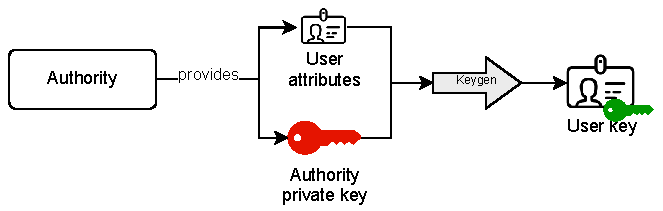
\includegraphics[width=\textwidth,height=0.7\textheight,keepaspectratio]{images/diagrams/keygen_diagram.pdf}
\caption{Key generation diagram. The authority generates a secret key and a public key, then uses the secret key to generate user keys based on attributes.}
\end{figure}
\end{frame}

% \begin{frame}
% \frametitle{Encryption process}
% \begin{itemize}
% \item To encrypt data, a user provides the system with the data to be encrypted, together with an access policy.
% \item The access policy is a boolean expression of attributes required to decrypt the data.
% \item A random symmetric key is generated and used to encrypt the data with AES.
% \item The same symmetric key is then encrypted using MA-ABE with the public keys of the authorities involved in the access policy.
% \item Both the encrypted symmetric key and the encrypted data are returned to the user.
% \end{itemize}
% \end{frame}

\begin{frame}
\frametitle{Encryption process}
\begin{figure}
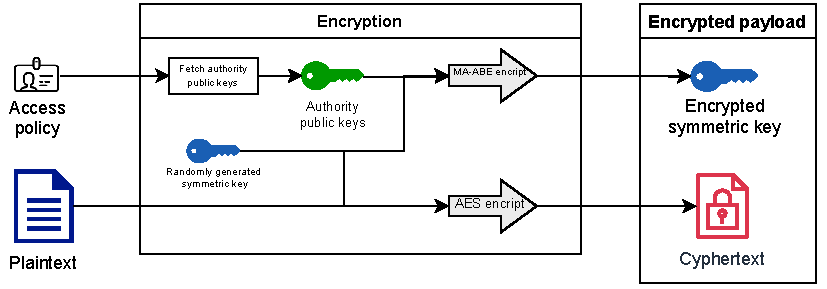
\includegraphics[width=\textwidth,height=0.7\textheight,keepaspectratio]{images/diagrams/encryption_diagram.pdf}
\caption{Encryption process diagram. The symmetric key is encrypted using MA-ABE, and the data is encrypted using AES.}
\end{figure}
\end{frame}

% \begin{frame}
% \frametitle{Decryption Process}
% \begin{itemize}
% \item To decrypt data, a user must possess a set of attribute keys that satisfies the access policy defined during encryption.
% \item The process first decrypts the symmetric key using the MA-ABE keys provided by the user and then uses the symmetric key to decrypt the payload with AES.
% \item This workflow enforces the access policy by requiring valid attribute keys to access the data.
% \end{itemize}
% \end{frame}

\begin{frame}
\frametitle{Decryption Process}
\begin{figure}
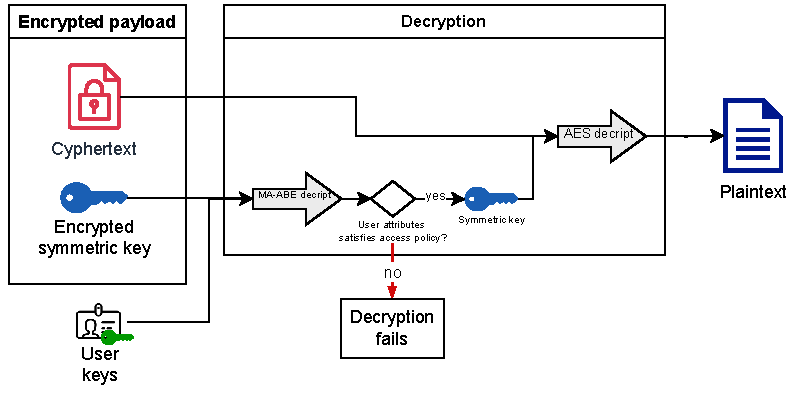
\includegraphics[width=\textwidth,height=0.7\textheight,keepaspectratio]{images/diagrams/decryption_diagram.pdf}
\caption{Decryption process diagram. The symmetric key is decrypted using MA-ABE, and the data is decrypted using AES.}
\end{figure}
\end{frame}

% --- Experimental Setup ---
\section{Experimental Setup}

\begin{frame}
\frametitle{Experimental Setup}
To validate our framework, we built and tested a complete prototype using a modern technology stack.

\begin{columns}[T] % The [T] option aligns the tops of the blocks
    \begin{column}{0.5\textwidth}
        \begin{block}{Core Components}
        \begin{itemize}
            \item \textbf{Cryptography:} Charm-Crypto with MaabeRW15 scheme
            \item \textbf{API Service:} Flask and Flask-RESTX
            \item \textbf{Key Storage:} Redis
        \end{itemize}
        \end{block}
    \end{column}
    
    \begin{column}{0.5\textwidth}
        \begin{block}{Testing and Infrastructure}
        \begin{itemize}
            \item \textbf{Load Testing:} Locust
            \item \textbf{Web Server:} Gunicorn
            \item \textbf{Reproducibility:} Docker
        \end{itemize}
        \end{block}
    \end{column}
\end{columns}

\end{frame}

% --- Results and Discussion ---
\section{Results and Discussion}

\begin{frame}
\frametitle{Evaluation Metrics}
We evaluated the system against several variables to measure its performance and scalability:
\begin{itemize}
    \item Server Concurrency (Workers \& Threads)
    \item Data Payload Size
    \item Simultaneous User Load
    \item Access Policy Complexity (Number of Attributes)
    \item User Key Storage Size
\end{itemize}
\end{frame}

\begin{frame}
\frametitle{Concurrency - Workers}
\begin{figure}
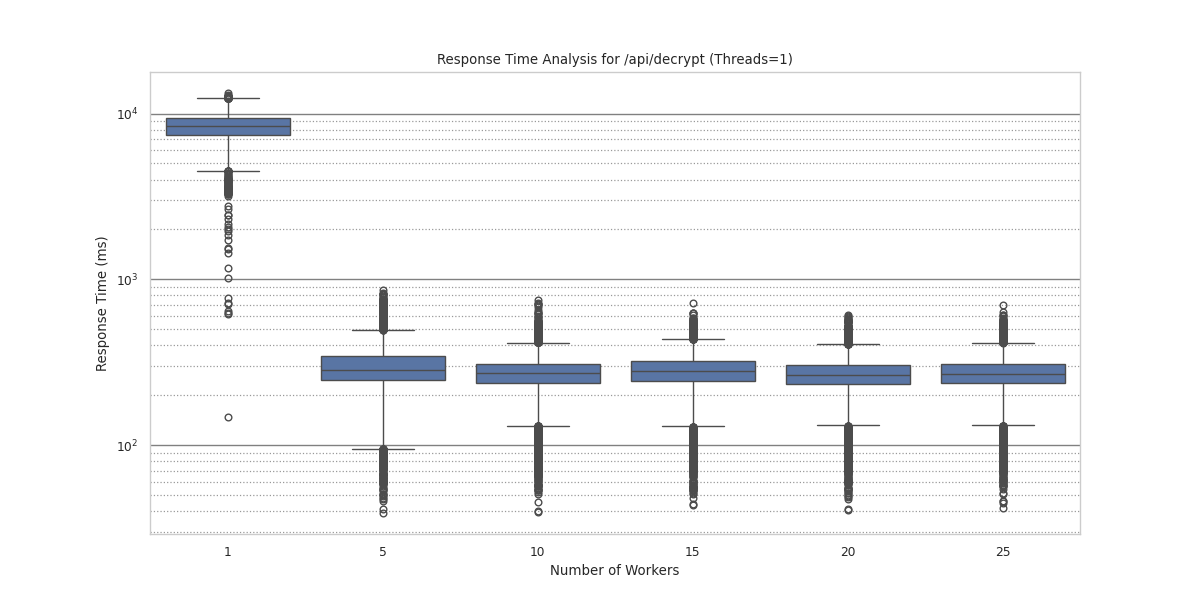
\includegraphics[width=\textwidth,height=0.75\textheight,keepaspectratio]{images/phase1/api_decrypt/response_time_threads_1.png}
\caption{Response time improves dramatically up to 5 worker processes and then stabilizes. This confirms the system scales effectively with processes, not threads.}
\end{figure}
\end{frame}

\begin{frame}
\frametitle{Concurrency - Threads}
\begin{figure}
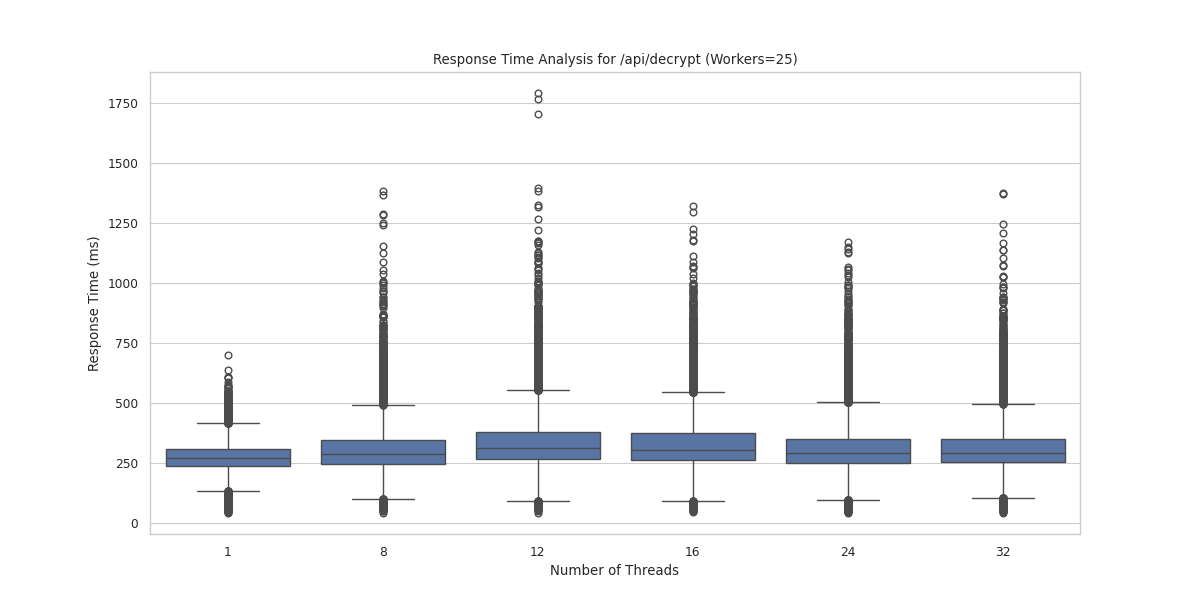
\includegraphics[width=\textwidth,height=0.75\textheight,keepaspectratio]{images/phase1/api_decrypt/response_time_workers_25.png}
\caption{The flat line demonstrates no performance gain from multi-threading. This is an expected result due to Python's Global Interpreter Lock (GIL).}
\end{figure}
\end{frame}

\begin{frame}
\frametitle{Impact of Payload Size - Encryption}
\begin{figure}
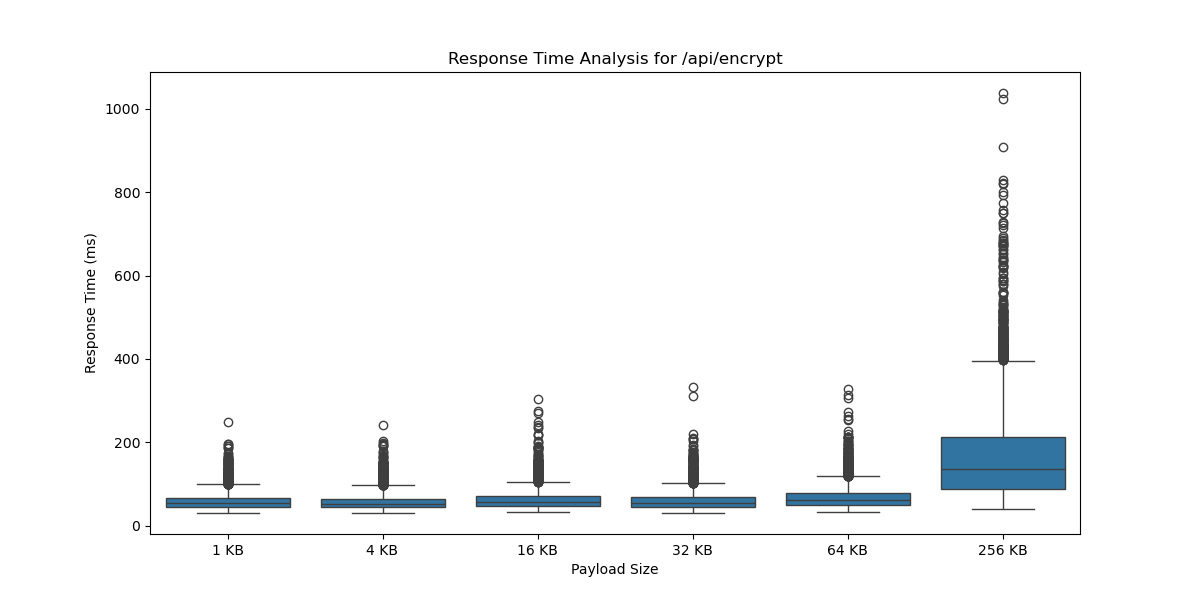
\includegraphics[width=\textwidth,height=0.75\textheight,keepaspectratio]{images/phase2/response_time_api_encrypt.png}
\caption{Encryption time scales linearly with payload size. This confirms the predictable and efficient performance of using AES for bulk data encryption.}
\end{figure}
\end{frame}

\begin{frame}
\frametitle{Impact of Payload Size - Decryption}
\begin{figure}
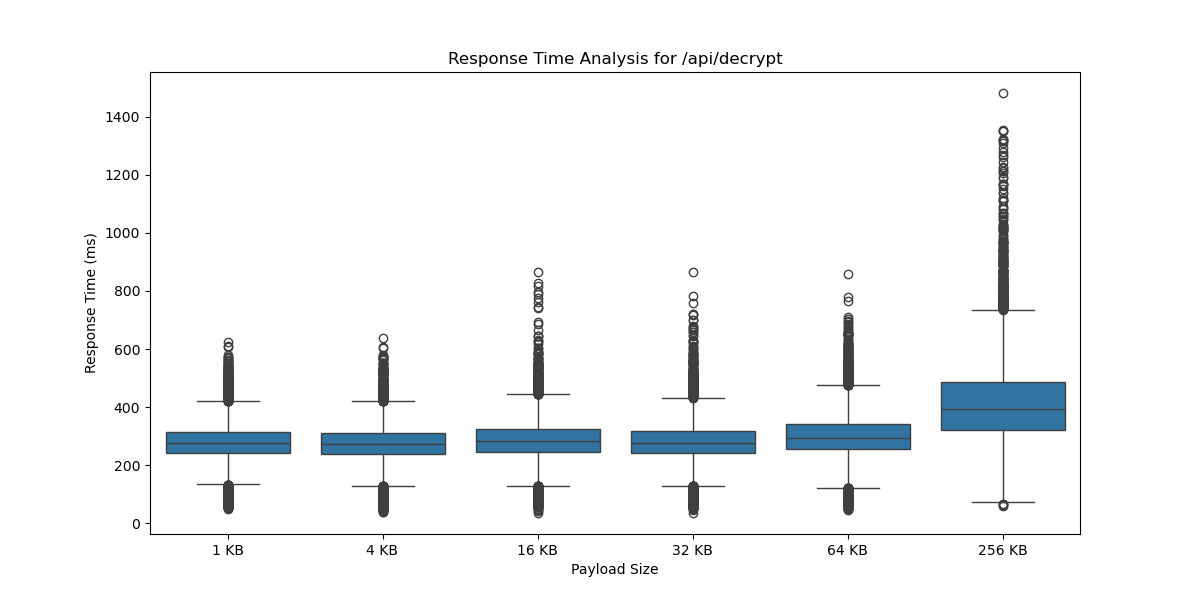
\includegraphics[width=\textwidth,height=0.75\textheight,keepaspectratio]{images/phase2/response_time_api_decrypt.png}
\caption{Decryption time also scales linearly. The higher time compared to encryption is due to the greater computational complexity of the decryption operation.}
\end{figure}
\end{frame}

\begin{frame}
\frametitle{Impact of User Load}
\begin{figure}
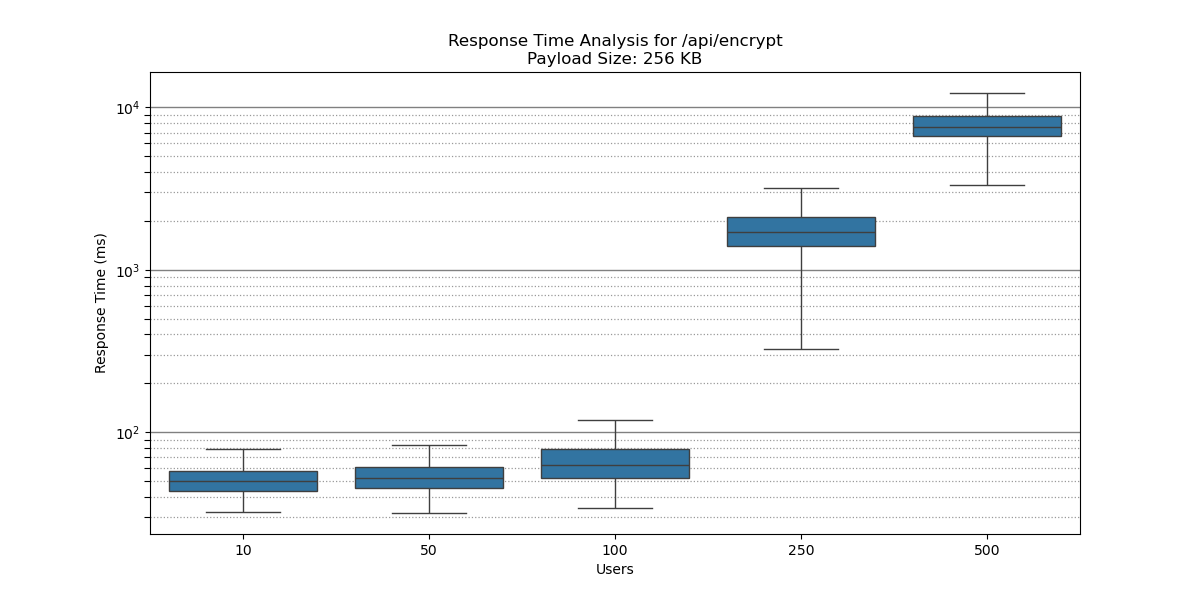
\includegraphics[width=\textwidth,height=0.75\textheight,keepaspectratio]{images/phase3/response_time_api_encrypt_256KB.png}
\caption{System response time remains stable and robust with up to 100 concurrent users. Above 100 users performance degrades due to memory constraints on the test bed machine.}
\end{figure}
\end{frame}

\begin{frame}
\frametitle{Impact of Policy Complexity}
\begin{figure}
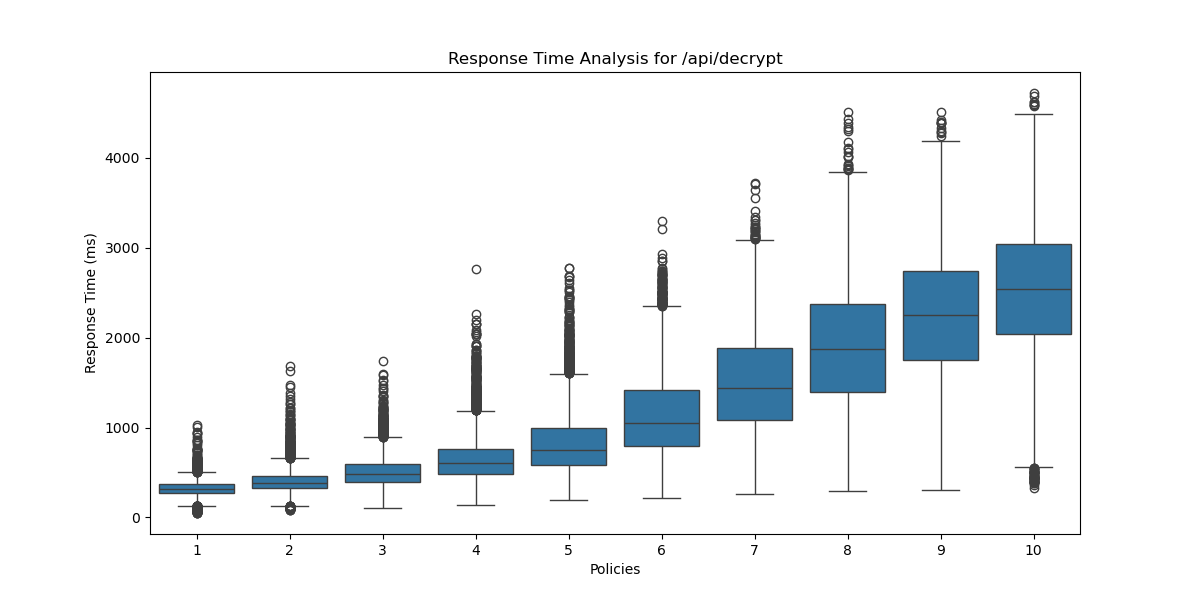
\includegraphics[width=\textwidth,height=0.75\textheight,keepaspectratio]{images/phase4/response_time_api_decrypt.png}
\caption{Decryption time increases significantly with more attributes in the policy. This highlights the direct trade-off between finer-grained security and performance.}
\end{figure}
\end{frame}

\begin{frame}
\frametitle{Impact of User Key Size}
\begin{figure}
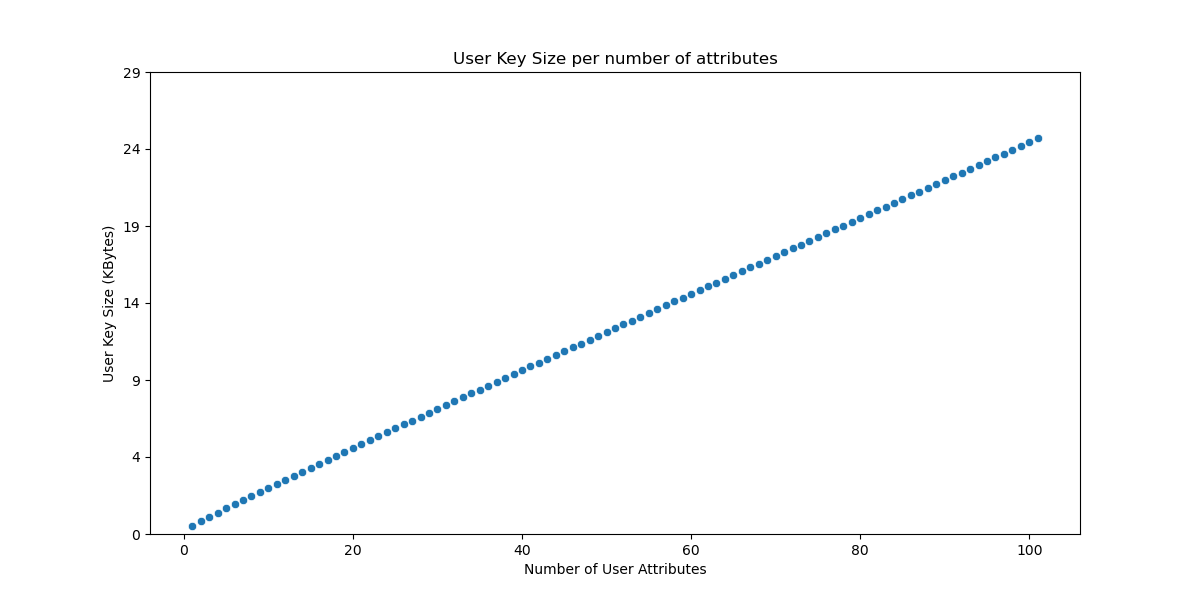
\includegraphics[width=\textwidth,height=0.75\textheight,keepaspectratio]{images/key_size_analysis/user_key_size_analysis.png}
\caption{The user's key storage size grows linearly with the number of attributes they possess, impacting storage requirements and I/O in attribute-heavy systems.}
\end{figure}
\end{frame}

% --- Conclusion ---
\section{Conclusion and Future Work}

\begin{frame}
\frametitle{Conclusion}
\begin{itemize}
    \item We successfully designed, implemented, and evaluated a hybrid MA-ABE and AES scheme for HIoT data security.
    \item Our evaluation confirmed the framework is a viable and effective solution for enforcing fine-grained access control in decentralized systems.
    \item The results provide valuable insights into the practical trade-offs between security, performance, and scalability for real-world deployment.
\end{itemize}
\end{frame}

\begin{frame}
\frametitle{Future Work}
\begin{itemize}
    \item \textbf{Full Integration and End-to-End Evaluation}
    \begin{itemize}
        \item Integrate the cryptographic framework with the target decentralized storage architecture and evaluate in a distributed environment.
    \end{itemize}
    \item \textbf{Performance and Efficiency Optimizations}
    \begin{itemize}
        \item Implement direct handling of binary data to reduce encoding overhead.
        \item Explore alternative key storage mechanisms to reduce I/O bottlenecks.
        \item Investigate hardware acceleration or parallel processing for MA-ABE operations.
    \end{itemize}
\end{itemize}
\end{frame}

\begin{frame}[allowframebreaks]
\frametitle{References}
\bibliography{biblio}
\end{frame}

% --- Thank you ---
\begin{frame}
\frametitle{Thank you!}
\begin{center}
\Large Questions?
\end{center}
\vspace{2cm}
\InfContacts
\end{frame}

\end{document}